\section{Discussion}
In the offline part, we analyzed the answers and video recordings of the C-subjects and found that 5 of them were close to the correct answers. In the C-task 1.1 and 1.2 they didn’t put so much effort. They were just looking for the matching actors and movies. Most of them answered the ones which they found at the beginning of the data. The ratings the C-subjects provided in the C-task 1.3 were based on their answer in C-task 1.1 and C-task 1.2. The C-subjects were given a short training which was a short version of C-task 234, C-task 3 and C-task 4. C-task 234 was based on the changing of patterns in the data which was performed well by all of the C-subjects. The technique they used was to find amount of dissimilarity between views of data for time t and time t+1. If time t+1 view do not contain any items of time t view or no heatmap signature in the previous timeline then it was highly probable that the P-subject has switched to another P-task.  Identifying which C-task they are looking at was comparatively easier. For C-task 2 and C-task 4, the clues were the corresponding movie names in the first time view. If none of them matches, they identified the task as C-task 3. For the recommendation task (C-task 2), all of the C-subjects followed an interesting method. The assumption is P-subjects answered their recommendation at the end of the task. So the C-subjects started looking at the end time for the C-task and went backward. They recommended the one which have a good heatmap signature throughout the task. Finding items for C-task 3 and C-task 4 was similar to the C-task 1.1 and 1.2. The C-subjects observed for longer time for C-task 3 and 4 than C-task 1.1 and 1.2. The reason behind this fact could be the C-subjects were little bit familiar with the analyzing tool. 

Next, the real-time part C-subjects were less accurate than the offline part C-subjects. They were pretty accurate on C-task 234 however some user missed to identify some P-tasks. The real-time C-subjects mainly were mostly incorrect on C-task 2. As the data was longer than the other tasks, the C-subject may have been impatient and answered the movies which they saw first. We calculated the correctness using the Sorensen-Dice coefficient~\cite{sorensen1948method}. The scatter plot on the correctness of C-subjects are plotted in Figure~\ref{fig:Scatter}.
\begin{figure}[htb]
  \centering
  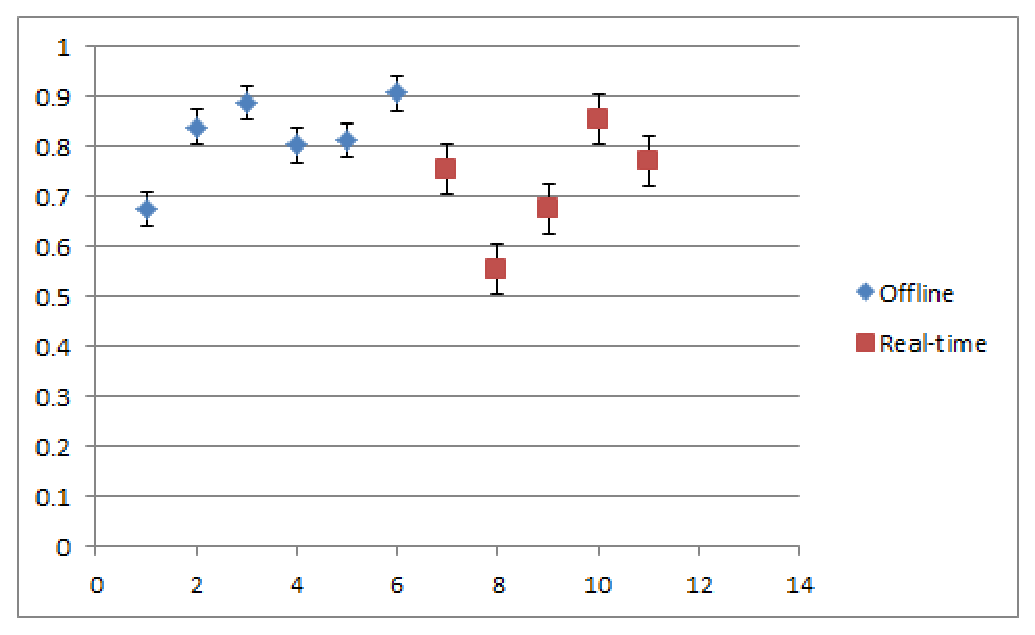
\includegraphics[width=0.9\linewidth]{images/Scatter.eps}
  \caption{Correctness of C-subjects in the C-study.}
	\label{fig:Scatter}
\end{figure} 